
\section{Fortbewegung}

\subsection{Fahrrad}

Fahrradfahren lohnt sich nicht nur, weil es die schnellste und
flexibelste Möglichkeit ist, in München voranzukommen, es ist auch
gesund, schont das Klima und macht Spaß.  Es ist auch deutlich
günstiger als die häufig überfüllten öffentlichen Nahverkehrsmittel:
Drei Monate Fahrrad statt MVG und schon hat man schnell um die 100~€
gespart.

Damit kann man schon den ein oder anderen Drahtesel refinanzieren oder
hat zumindest eine Anzahlung für ein gutes, gebrauchtes Fahrrad. Diese
findet man beispielsweise bei eBay, Polizei-, Bahnhofs- und
Wohnheimversteigerungen oder auf einem der zahlreichen Flohmärkte in
München. Kleiner Tipp: Beschränke dich bei der Suche nicht nur auf die
Stadt, sondern beziehe das Umland mit ein. Dort findet man oft
deutlich bessere Angebote.

München ist nicht nur Radlhauptstadt, sondern auch (gefühlte) Kontrollierhauptstadt. Auf ausgeschilderten Strecken Schrittgeschwindigkeit einhalten, sonst zahlt man schnell 15~€. Auf der falschen Straßenseite fahren (dies gilt auch auf der Leopold- / Ludwigstr) sowie ohne Licht bei Nacht oder Dunkelheit kosten 20~€.
Vor allem nicht unterschätzen sollte man das Rotlicht an Ampeln. Durch ignorieren dieses ist man schnell mal 100~€ los und hat zusätzlich noch Punkte in Flensburg.

\paragraph{Hier noch ein paar Tipps für den Münchner Straßenverkehr:}
\begin{itemize}
	\item Um Trambahnschienen sollte man nicht nur bei Regen und Glätte einen großen Bogen machen.
	\item Fußgänger sind in ihrem Verhalten unvorhersehbar. Die Autofahrer leider auch.
	\item Mit Helm fahren kann dein Leben retten.
	\item Um das Wiederfinden des Fahrrades zu erleichtern, sollte man es abschließen.
	
\end{itemize}

%\begin{textblock*}{\paperwidth}(50mm,128mm)
%   \noindent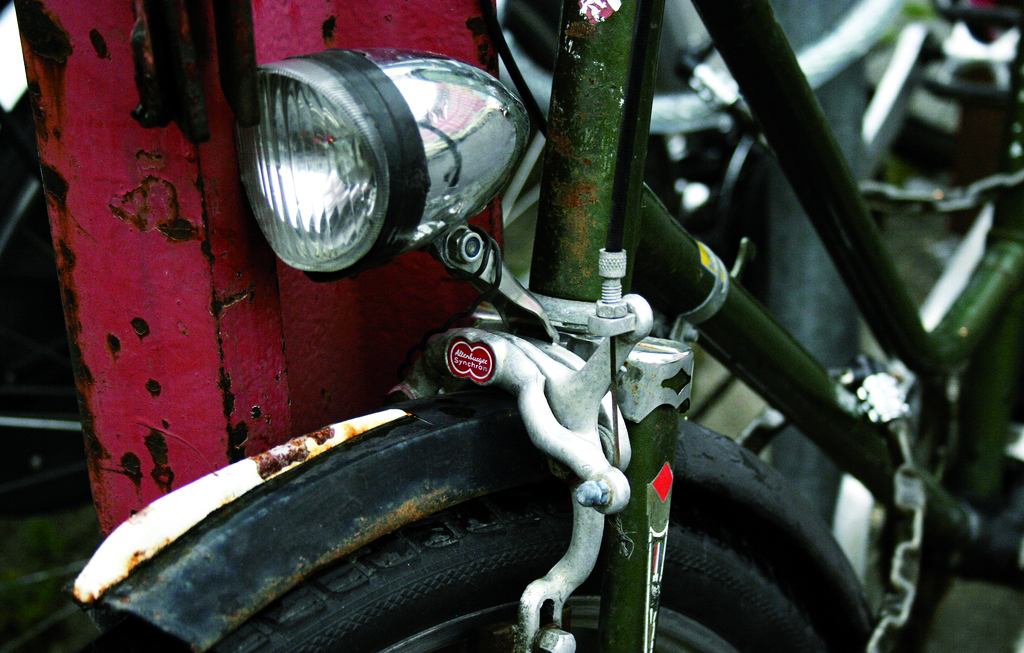
\includegraphics[width={\paperwidth-50mm}]{flickr/725703538_5b9a97ecf2_b}
%	\label{img_bike}
%\end{textblock*}

\clearpage

\subsection{MVV}

\paragraph{Mit den öffentlichen Verkehrsmitteln in die Uni}\hfill\\
Die U-Bahnen U3 und U6 halten direkt am Hauptgebäude (Haltestelle Universität). Die meisten anderen Gebäude sind ebenfalls mit U-Bahn, Bus oder Tram gut zu erreichen. Genaueres zu den wichtigsten Gebäuden und naheliegenden Haltestellen finden sich auf der in der Mitte dieses Heftes zu findenden Karte.

%\paragraph{Kosten}\hfill\\
%Für die meisten Studika ist momentan der von der MVV (Münchner Verkehrsverbund) angebotene Ausbildungstarif II am interessantesten. Der Preis richtet sich dabei nach der Zahl der benötigten Zeitkartenringe, die befahren werden. Bevor du dir aber ein Ticket kaufen kannst, musst du dir ein Kundenkarte besorgen. Diese bekommst du im MVG-Kundencenter am Hauptbahnhof, Ostbahnhof oder in der Poccistr.~1--3 (alle zwischen 8:00 und 18:00~Uhr) oder online \newline http://www.mvv-muenchen.de/de/tickets-preise/tickets/schule-ausbildung-und-studium/\newline kundenkarte/index.html\#c9815

%Das Ticket gibt es mit der Gültigkeit einer Woche (9,50 -- 38,90~€) oder eines Monats (34,70 -- 142,00~€) an einem der MVG-Zeitkartenautomaten, in den MVG-Kundencentern oder den MVG-Verkaufsstellen. Monatsfahrkarten gelten bis 12Uhr des ersten Werktags des Folgemonats.\\
%~
%Wenn du in Zukunft günstiger unterwegs sein willst, kannst du bei der Initiative Ausbildungsticket, einem Bündnis aus Studika, Schülern und Azubis mitmachen:\newline \url{ausbildungsticket.de}

%Mehr Infos zum Ausbildungstarif: \url{mvg-mobil.de/tarife/ausbildungstarif.html}


\subsection{Auto}
Du kommst im Allgemeinen mit dem Auto nicht schneller durch die Stadt, als mit dem ÖPNV oder dem Fahrrad. Spätestens bei der Parkplatzsuche vor der Uni wirst du dann merken, dass es bessere Möglichkeiten gibt, an die Uni zu kommen.
